\documentclass[10pt,a4paper]{article}

\usepackage[utf8]{inputenc}
\usepackage[T1]{fontenc}
\usepackage[italian]{babel}
\usepackage{graphicx}
\usepackage{amsmath,amssymb,amsfonts}
\usepackage{caption}
\usepackage{subcaption}
\usepackage{wrapfig}
\usepackage{float}
\usepackage{geometry}
\geometry{top=2.5cm, bottom=2.5cm, left=1.7cm, right=1.7cm}
\usepackage{fancyhdr}
\usepackage{titlesec}
\usepackage{lmodern}
\usepackage{caption}
\usepackage{comment}
\usepackage{booktabs}
\usepackage{makecell}
\usepackage{siunitx}
\usepackage{bm}
\usepackage[version=4]{mhchem} 
\DeclareCaptionFont{myit}{\footnotesize\itshape\fontfamily{cmr}\selectfont}
\captionsetup{
    font=myit,
    labelfont={bf},
    textfont=normalfont
}
\usepackage{titletoc}

% Intestazioni moderne
\pagestyle{fancy}
\fancyhf{}
\fancyhead[L]{Vita media del $\mu$}
\fancyhead[R]{Niccolò Menichetti \\ Luca Musetti \\ Luca Nasone}
\fancyfoot[C]{\thepage}

% Re e Im
\renewcommand{\Re}{\mathop{\mathrm{Re}}}
\renewcommand{\Im}{\mathop{\mathrm{Im}}}

% Per "simulare" capitoli
\newcommand{\chapter}[1]{
    \clearpage
    \section*{#1}
    \addcontentsline{toc}{section}{#1}
}

\title{\bfseries Relazione di laboratorio \\[1ex] \Large Vita media del $\mu$}
\author{Niccolò Menichetti \\ Luca Musetti \\ Luca Nasone}
\date{Anno Accademico 2025--2026}

\begin{document}

\begin{titlepage}
    \thispagestyle{empty}
    
    \begin{figure}[ht]
        \centering
        \begin{minipage}{0.48\textwidth}
            \centering
            
\includegraphics[width=5.0cm]{Immagini/Stemma_unipi.svg.png}
        \end{minipage}%
        \hfill
        \begin{minipage}{0.48\textwidth}
            \centering
            
\includegraphics[width=7.0cm]{Immagini/unipi_fermi.png}
        \end{minipage}
    \end{figure}

    \vspace{4.0cm} % Spazio per centrare verticalmente il contenuto

    \begin{center}
        {\fontsize{20pt}{24pt}\selectfont\bfseries Vita media del muone}\\[0.3cm]
        {\large Relazione laboratorio di interazioni fondamentali}\\[9.0cm]

        {\Large NICCOLO' MENICHETTI\hspace{0.2cm} LUCA MUSETTI \hspace{0.2cm} LUCA NASONE}\\[0.35cm]
        {\normalsize Anno Accademico 2025 - 2026}
    \end{center}

\end{titlepage}

\newpage


\begin{abstract}
        
    \emph{Nella seguente relazione descriviamo la nostra misura della vita media del muone, effettuata sui muoni dei raggi cosmici. Otteniamo una vita media pari a ...(To be continued...)}
        
\end{abstract}

\tableofcontents

\newpage

\section{Introduzione}

Sappiamo che, a causa dell'interazione con l'atmosfera, i raggi cosmici che arrivano dallo spazio hanno una composizione differente a livello del mare. In particolare prevalgono i muoni $\mu$, che decadono nel seguente modo:

\begin{equation}
    \ce{$\mu^{-}\rightarrow e^{-}\bar \nu_e \nu_{\mu}$}
\end{equation}


con vita media è $\tau_{\mu} = 2.1969811 \pm 0.0000022 $ $\mu s$ (PDG 2025) e carica $\pm e$.

L'obiettivo dell'esperimento è misurare il valore della vita media del muone, con un apparato sperimentale in grado di rilevare i raggi cosmici e fermare i $\mu$ a bassa energia. 

Nella materia i muoni negativi tendono a formare degli stati legati con i nuclei (atomi mesici). Questo fatto rende la vita media del muone con carica negativa più bassa di quella per muoni con carica positiva. Con i dati a nostra disposizione possiamo estrarre l'abbondanza relativa di una specie rispetto all'altra, ossia $N_+/N_-$, note le popolazioni $N_+$ e $N_-$ per i muoni con la carica $\pm e$ rispettivamente.

Utilizzando gli impulsi rilasciati nei fotomoltiplicatori, è stato possibile, previa un'opportuna calibrazione, misurare lo spettro in energia dell'$e^{-}$ prodotto dal decadimento. Essendo un decadimento a 3 corpi, sappiamo che per certo non è monocromatico, ma si ricava facilmente dalla cinematica relativistica che è limitato superiormente da:

\begin{equation}
    E_e^{max} = \frac{m_{\mu}^2+m_{e}^2}{2m_{\mu}}\approx\frac{m_{\mu}}{2}
\end{equation}

l'ultima approssimazione usa il fatto che $m_{\mu}\gg m_e$.

Usando $m_\mu = 105.6583755 \pm 0.0000023$ MeV (PDG 2025), tale valore corrisponde a $52.82918775 \pm 0.00000011$. Un calcolo più approfondito mostra che tale valore è anche il massimo della distribuzione in energia dell'elettrone. Lo spettro risultante dunque cresce fino a tale valore e si annulla con una discontinuità per energie maggiori. 

Di conseguenza con una misura di spettro è possibile trovare tale punto di discontinuità e dall'equazione (2) la massa del muone.

%Vedi se mettere anche la massa dell'elettrone per essere più formale, e vedi se troncare le cifre significative

\section{Apparato sperimentale}

\begin{figure}[h]
\centering
\begin{minipage}{0.40\textwidth}
    \centering
    \includegraphics[width=0.55\textwidth]{Immagini/telescopio.jpeg}
    \caption{Sistema Telescopio+Blocco+VETO}
\end{minipage}
\begin{minipage}{0.4\textwidth}
    \centering
    \includegraphics[width=0.55\textwidth]{Immagini/Circuito.jpeg}
    \caption{Apparato di lettura dei segnali ricevuti dai PMT}
\end{minipage}
\end{figure}

\begin{itemize}
\item 6 lastre di scintillatore lette ciascuno da un fotomoltiplicatore (PMT), dimensioni (49.8 $\pm$ 0.1 cm) $\times$ (27.5 $\pm$ 0.1 cm) $\times$ (2.3 $\pm$ 0.1 cm);
\item 1 blocco di scintillatore letto da 4 PMT, dimensioni (30.0 $\pm$ 0.1 cm) $\times$ (31.0 $\pm$ 0.1 cm) $\times$ (31.0 $\pm$ 0.1) ;
\item una scheda DE0-10 NANO;
\item 2 discriminatori (NIM CAEN N84 e NIM INFN);
\item 3 unità di coincidenza (NIM LRS 465, NIM CERN N6234, NIM INFN);
\item 1 unità di OR (NIM CERN);
\item 2 unità di Dual Timer (NIM CAEN mod2255B e NIM CAEN N2255);
\item 1 unità di conversione NIM-TTL (NIM INFN);
\item 1 multiscaler (NIM INFN Multiscaler130);
\item 1 unità di Fan-Out (NIM CERN);
\item 1 integratore analogico (NIM CAEN N914);
\item 1 ADC (NIM CAEN N6725);
\item 1 oscilloscopio (Tektronix TBS1104);
\item 2 computer, per regolare le alimentazioni e per le acquisizioni;
\item 1 multimetro (Fluke);
\item cavi coassiali di vario ritardo;
\item terminazioni a 50 e 0 $\Omega$;
\item 1 metro a nastro;
\end{itemize}

\newpage

\section{Punto di lavoro}

\subsection{Telescopio}

Le misure iniziali sono state volte a scegliere il punto di lavoro dei vari PMT. Soglie e alimentazioni influenzano l'efficienza e di conseguenza il numero di eventi rivelati. Vogliamo sia più alta possibile in modo da massimizzare la statistica a nostra disposizione. 

Sono stati scelti il PMT07, il PMT04 e il PMT02. Per ogni PMT (poniamo, ad esempio il PMT07)abbiamo misurato il rapporto fra le coincidenze triple $(07\land04\land02)$ e le coincidenze doppie degli altri due (nel nostro esempio $(04\&02)$). 

Misuriamo i conteggi delle coincidenze fra i segnali discriminati per 100 s tramite il multiscaler. Tale misura viene poi ripetuta variando l'alimentazione. 

Durante la procedura sono state misurate anche le singole dei due PMT usati per le coincidenze doppie, in quanto il loro rate in singola influenza il numero di doppie false $D_{fake}$, ottenuto da:

\begin{equation}
D_{fake} = R_1 R_2 \Delta t (w_1 + w_2 - 2w) 
\end{equation}

Dove $R_1$ e $R_2$ sono i rate in singola dei PMT di interesse, $w_1$ e $w_2$ sono le durate dei loro segnali discriminati (50 ns nel nostro caso). $w$ è la sovrapposizione temporale minima per avere una coincidenza, di 2 ns. Sceglieremo alimentazioni e soglie cercando di rendere il numero di doppie false trascurabile rispetto alle doppie misurate.

Tale procedura è ottimale per il PMT04, ma non per il PMT07 e PMT02, a causa della geometria del sistema. 
Per correggere tale effetto abbiamo usato un metodo Montecarlo per simulare il passaggio dei raggi cosmici attraverso il rivelatore, al fine di ricavare la probabilità che un raggio cosmico passi per un PMT dato il passaggio dagli altri due (accettanza). 
Dividendo il rapporto triple su doppie misurato con tale valore si ottiene una stima dell'efficienza.

Stimiamo l'errore sul rapporto triple su doppie con: 

\begin{equation}
\sigma_{\varepsilon} = \sqrt{\frac{\varepsilon(1-\varepsilon)}{D}}
\end{equation}

$D$ è il numero di doppie.

Riportiamo di seguito le curve di efficienza, con le misure effettuate (alimentazione, efficienza, errore sull'efficienza e numero di doppie false) nella tabella accanto:

\begin{figure}[H]
\centering

\begin{minipage}{0.48\textwidth}
    \centering
    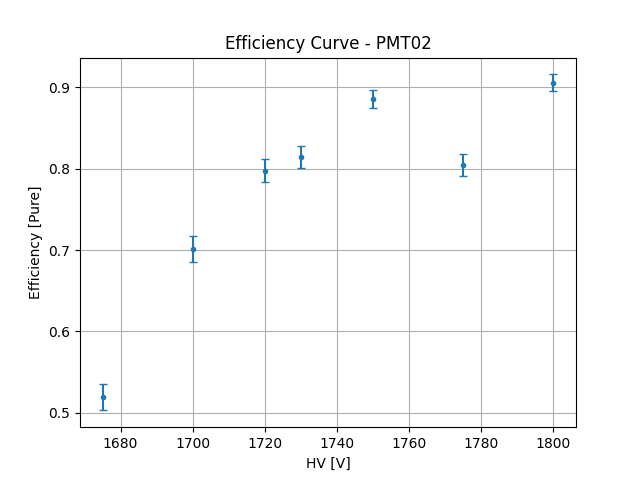
\includegraphics[width=\linewidth]{Grafici/Efficiency Curves - PMT02.png}
    \caption{Curva di efficienza PMT02}
\end{minipage}
\hfill
\begin{minipage}{0.48\textwidth}
    \centering
    \textbf{PMT02}

    \vspace{0.25cm}

    \begin{tabular}{cccc}
    \toprule
    $HV$[V] ($\pm$ 1V) & $\varepsilon$ [$\%$] & $\sigma_{\varepsilon}$[$\%$] & $D_{fake}$ \\
    \midrule
    1675 & 52 & $\pm$ 2 & 0.69 \\
    1700 & 70 & $\pm$ 2 & 0.65 \\
    1720 & 80 & $\pm$ 1 & 0.63 \\
    1730 & 81 & $\pm$ 1 & 0.59 \\
    1750 & 89 & $\pm$ 1 & 0.53 \\
    1775 & 80 & $\pm$ 1 & 0.54 \\
    1800 & 91 & $\pm$ 1 & 0.56 \\
    \bottomrule
    \end{tabular}
    \captionof{table}{Misure effettuate per il PMT02}
\end{minipage}

\end{figure}


\begin{figure}[H]
\centering

\begin{minipage}{0.48\textwidth}
    \centering
    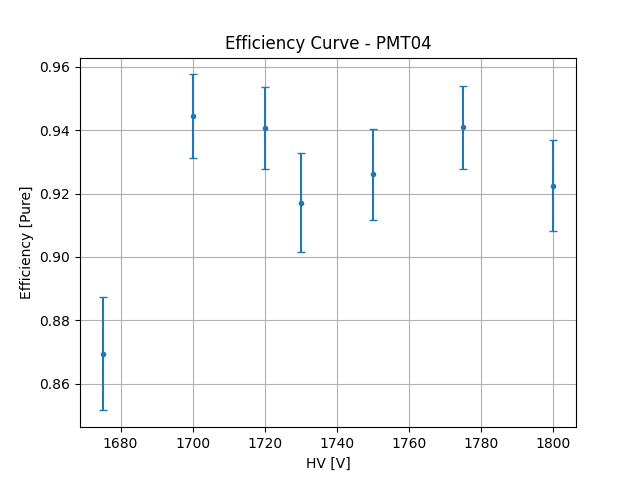
\includegraphics[width=\linewidth]{Grafici/Efficiency Curves - PMT04.png}
    \caption{Curva di efficienza PMT04}
\end{minipage}
\hfill
\begin{minipage}{0.48\textwidth}
    \centering
    \textbf{PMT04}

    \vspace{0.25cm}
    
    \begin{tabular}{cccc}
    \toprule
    $HV$[V] ($\pm$ 1V)& $\varepsilon$ [$\%$] & $\sigma_{\varepsilon}$[$\%$] & $D_{fake}$ \\
    \midrule
    1675 & 87 & $\pm$ 2 & 0.077 \\
    1700 & 94 & $\pm$ 1 & 0.068 \\
    1720 & 94 & $\pm$ 1 & 0.074 \\
    1730 & 92 & $\pm$ 2 & 0.073 \\
    1750 & 93 & $\pm$ 1 & 0.078 \\
    1775 & 94 & $\pm$ 1 & 0.076 \\
    1800 & 92 & $\pm$ 1 & 0.076 \\
    \bottomrule
    \end{tabular}
    \captionof{table}{Misure effettuate per il PMT04}
\end{minipage}

\end{figure}

\begin{figure}[H]
\centering

\begin{minipage}{0.48\textwidth}
    \centering
    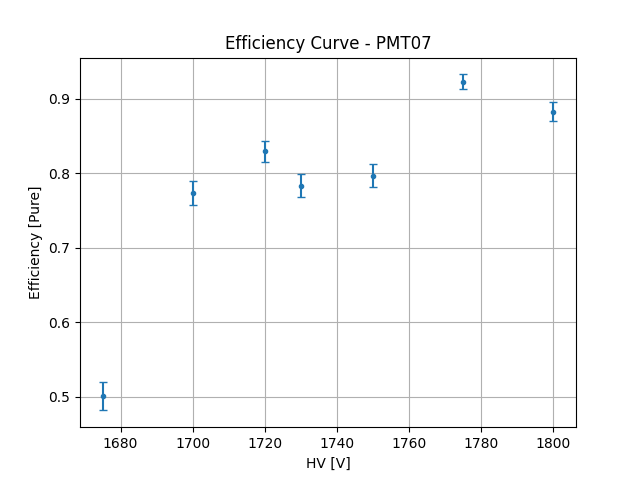
\includegraphics[width=\linewidth]{Grafici/Efficiency Curves - PMT07.png}
    \caption{Curva di efficienza PMT07}
\end{minipage}
\hfill
\begin{minipage}{0.48\textwidth}
    \centering
    \textbf{PMT07}

    \vspace{0.25cm}
    
    \begin{tabular}{cccc}
    \toprule
    $HV$[kV] ($\pm$ 1V)& $\varepsilon$ [$\%$] & $\sigma_{\varepsilon}$[$\%$] & $D_{fake}$ \\
    \midrule
    1.675 & 50 & $\pm$ 2 & 0.97 \\
    1.700 & 77 & $\pm$ 2 & 0.79 \\
    1.720 & 83 & $\pm$ 1 & 0.73 \\
    1.730 & 78 & $\pm$ 2 & 0.73 \\
    1.750 & 80 & $\pm$ 2 & 0.68 \\
    1.775 & 92 & $\pm$ 1 & 0.64 \\
    1.800 & 88 & $\pm$ 1 & 0.57 \\
    \bottomrule
    \end{tabular}
    \captionof{table}{Misure effettuate per il PMT07}
\end{minipage}

\end{figure}


\vspace{1.2cm}

In conclusione il punto di lavoro scelto per il telescopio è:

\begin{center}
\vspace{0.6cm}

\begin{tabular}{cccc}
\toprule
Parametro & PMT02 & PMT04 & PMT07 \\
\midrule
$V_{supply}$ [V] & 1750 & 1700 & 1750 \\
$V_{thr}$ [mV] & -30 & -30 & -30 \\
$\varepsilon$ [$\%$] & 88 & 94 & 79 \\
\bottomrule
\end{tabular}
\captionof{table}{Punto di lavoro scelto per il telescopio}
\end{center}

\subsection{Bersaglio}

Abbiamo ricostruito la curva di efficienza anche per i PMT del bersaglio. 
Al fine di creare una geometria favorevole alla misura, abbiamo usato diverse combinazioni di scintillatori in modo che il rivelatore di cui si voleva misurare l'efficienza risultasse posizionato in mezzo agli altri due.

Riportiamo le combinazioni usate per ciascun PMT del blocco:

\begin{itemize}

\item PMT08 : PMT02-PMT08-PMT10 
\item PMT09 : PMT02-PMT09-PMT01
\item PMT10 : PMT07-PMT08-PMT10
\item PMT11 : PMT09-PMT11-PMT01

\end{itemize}

Per PMT08-09-11 si è usato il metodo dei trigger ortogonali con lo scintillatore immediatamente sopra/sotto.

Il PMT10 è fuori asse col PMT01, quindi non ci è sembrato ragionevole usare tale procedura. Invece usiamo il PMT08 e il PMT07. Vogliamo infatti massimizzare la probabilità che dato il passaggio nei due PMT soprastanti si abbia il passaggio anche nel blocco. Un calcolo mostra che tale probabilità $P$ corrisponde a: 
\begin{equation}
P = \frac{1- cos(\theta_1)}{1- cos(\theta_2)}
\end{equation}
$\theta_1$ e $\theta_2$ sono gli angoli massimi accettati da telescopio e bersaglio. Da cui si vede che la condizione ottimale è che $\theta_2\rightarrow0$, con $\theta_2\approx \frac{l}{D}$, $l$ la larghezza dello scintillatore e $D$ la distanza fra lo stesso e il bersaglio. Dunque massimizzando $D$ si aumenta la probabilità, da cui la scelta dei PMT.

Per il resto, le misure di rate si sono svolte come descritto nella sezione precedente, così come le stime di errore.

Riportiamo come sopra grafico e misure in tabella:

\begin{figure}[H]
\begin{minipage}{0.48\textwidth}
    \centering
    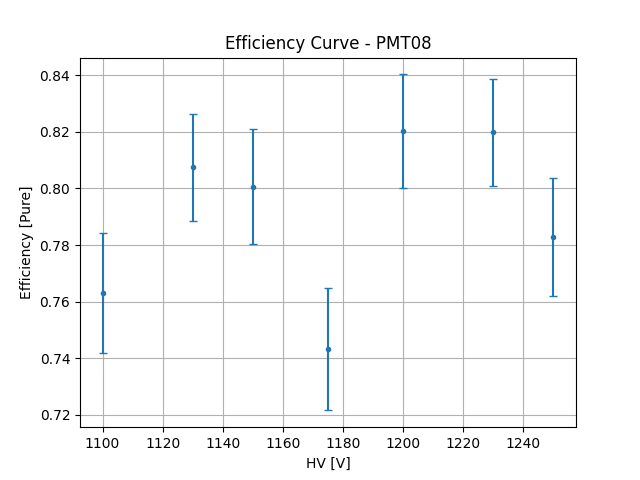
\includegraphics[width=\linewidth]{Grafici/Efficiency Curves - PMT08.png}
    \caption{Curva di efficienza PMT08}
\end{minipage}
\hfill
\begin{minipage}{0.48\textwidth}
    \centering
    \textbf{PMT08}

    \vspace{0.25cm}
    
    \begin{tabular}{cccc}
    \toprule
    HV [V] ($\pm$ 1 V)& $\varepsilon [\%]$ & $\sigma_{\varepsilon} [\%]$ & $D_{fake}$ \\
    \midrule
    1100 & 76 & $\pm$ 2 & 0.01 \\
    1130 & 81 & $\pm$ 2 & 0.02 \\
    1150 & 80 & $\pm$ 2 & 0.02 \\
    1175 & 74 & $\pm$ 2 & 0.03 \\
    1200 & 82 & $\pm$ 2 & 0.04 \\
    1230 & 82 & $\pm$ 2 & 0.06 \\
    1250 & 78 & $\pm$ 2 & 0.07 \\
    \bottomrule
    \end{tabular}
    \captionof{table}{Misure effettuate per il PMT08}
\end{minipage}
\begin{minipage}{0.48\textwidth}
    \centering
    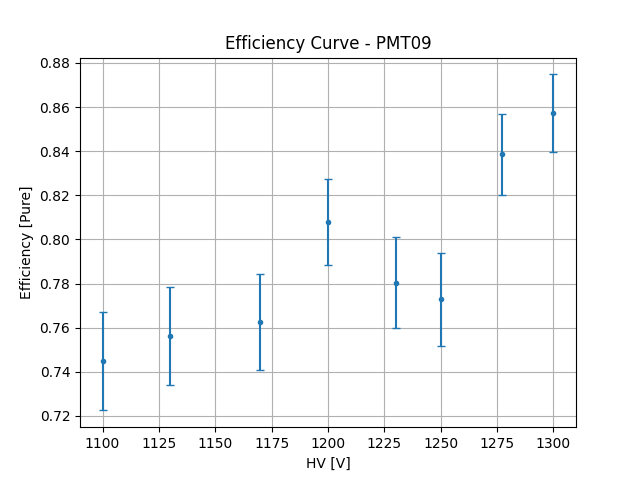
\includegraphics[width=\linewidth]{Grafici/Efficiency Curves - PMT09.png}
    \caption{Curva di efficienza PMT09}
\end{minipage}
\hfill
\begin{minipage}{0.48\textwidth}
    \centering
    \textbf{PMT09}

    \vspace{0.25cm}
    
    \begin{tabular}{cccc}
    \toprule
    HV [V] ($\pm$ 1V) & $\varepsilon [\%]$ & $\sigma_{\varepsilon} [\%]$ & $D_{fake}$ \\
    \midrule
    1100 & 75 & $\pm$ 2 & 0.080 \\
    1130 & 76 & $\pm$ 2 & 0.076 \\
    1170 & 76 & $\pm$ 2 & 0.077 \\
    1200 & 81 & $\pm$ 2 & 0.077 \\
    1230 & 78 & $\pm$ 2 & 0.078 \\
    1250 & 77 & $\pm$ 2 & 0.079 \\
    1277 & 84 & $\pm$ 2 & 0.077 \\
    1300 & 86 & $\pm$ 2 & 0.079 \\
    \bottomrule
    \end{tabular}
   
    \captionof{table}{Misure effettuate per il PMT09}
\end{minipage}
\end{figure}


\begin{figure}[H]
\begin{minipage}{0.48\textwidth}
    \centering
    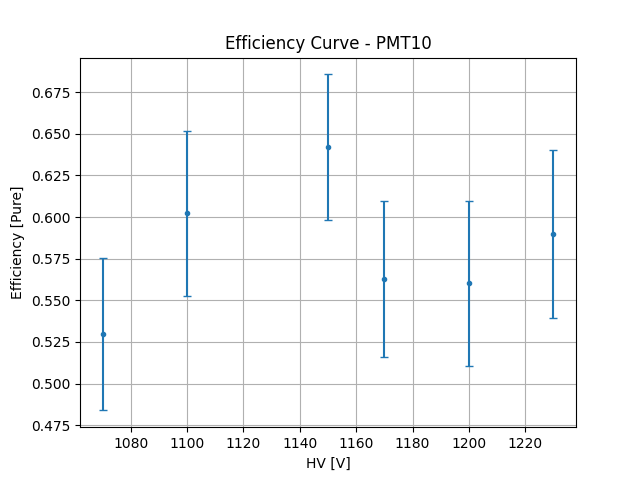
\includegraphics[width=\linewidth]{Grafici/Efficiency Curves - PMT10.png}
    \caption{Curva di efficienza PMT10}
\end{minipage}
\hfill
\begin{minipage}{0.48\textwidth}
    \centering
    \textbf{PMT10}

    \vspace{0.25cm}
    
    \begin{tabular}{cccc}
    \toprule
    HV [V] ($\pm$ 1V) & $\varepsilon [\%]$ & $\sigma_{\varepsilon} [\%]$ & $D_{fake}$ \\
    \midrule
    1070 & 53 & $\pm$ 5 & 0.054 \\
    1100 & 60 & $\pm$ 5 & 0.047 \\
    1150 & 64 & $\pm$ 4 & 0.055 \\
    1170 & 56 & $\pm$ 5 & 0.054 \\
    1200 & 56 & $\pm$ 5 & 0.059 \\
    1230 & 59 & $\pm$ 5 & 0.054 \\
    \bottomrule
    \end{tabular}
   
    \captionof{table}{Misure effettuate per il PMT10}
\end{minipage}
\begin{minipage}{0.48\textwidth}
    \centering
    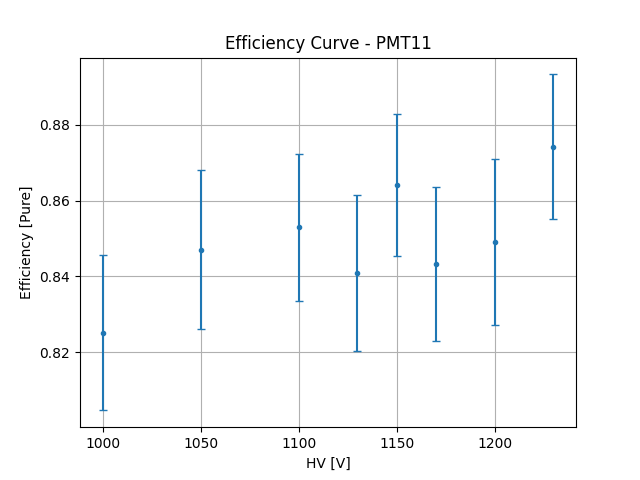
\includegraphics[width=\linewidth]{Grafici/Efficiency Curves - PMT11.png}
    \caption{Curva di efficienza PMT11}
\end{minipage}
\hfill
\begin{minipage}{0.48\textwidth}
\centering
    \textbf{PMT11}
    
    \vspace{0.25cm}
    
    \begin{tabular}{cccc}
    \toprule
    HV [V] ($\pm$ 1V) & $\varepsilon [\%]$ & $\sigma_{\varepsilon} [\%]$ & $D_{fake}$ \\
    \midrule
    1100 & 74 & $\pm$ 2 & 0.077 \\
    1130 & 76 & $\pm$ 2 & 0.077 \\
    1170 & 76 & $\pm$ 2 & 0.077 \\
    1200 & 81 & $\pm$ 2 & 0.077 \\
    1230 & 78 & $\pm$ 2 & 0.077 \\
    1250 & 79 & $\pm$ 2 & 0.079 \\
    1277 & 84 & $\pm$ 2 & 0.080 \\
    1300 & 86 & $\pm$ 2 & 0.079 \\
    \bottomrule
    \end{tabular}

    \captionof{table}{Misure effettuate per il PMT11}
\end{minipage}

\end{figure}

Il punto di lavoro scelto è stato dunque:

\begin{center}
\begin{tabular}{ccccc}
\toprule
Parametro & PMT08 & PMT09 & PMT10 & PMT11 \\
\midrule
$V_{supply}$ [V] & 1260  & 1320  & 1260  & 1260  \\
$V_{thr}$ [mV] & -80 & -80 & -80 & -80 \\
$\varepsilon$ [$\%$] & 78  & 85  & 58 & 87 \\
\bottomrule
\end{tabular}
\captionof{table}{Punto di lavoro scelto per il bersaglio}

\end{center}


\subsection{VETO}

Infine abbiamo eseguito lo studio analogo per il PMT01(VETO). Abbiamo usato il rapporto triple su doppie della terna PMT07 - PMT09 $\vee$ PMT11 - PMT01. 

Il ragionamento per la scelta della terna di PMT è lo stesso del caso precedente del PMT10, in quanto non è presente uno scintillatore sottostante al PMT01, dunque il metodo dei trigger ortogonali non ci è risultato ottimale per la misura.
Riportiamo sempre grafico e tabella: 


\begin{figure}[H]
\centering

\begin{minipage}{0.52\textwidth}
\centering
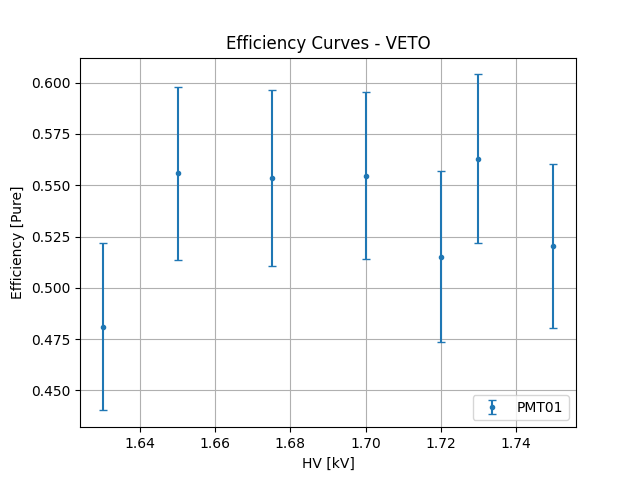
\includegraphics[width=\linewidth]{Grafici/Efficiency Curves - VETO.png}
\caption{Curva di efficienza per il PMT01}
\label{fig:veto_efficiency}
\end{minipage}
\hfill
\begin{minipage}{0.42\textwidth}
\centering
\textbf{PMT01}

\vspace{0.25cm}

\begin{tabular}{|r|r|r|r|}
\toprule
HV [kV] & $\varepsilon [\%]$ & $\sigma_{\varepsilon} [\%]$ & $D_{fake}$ \\
\midrule
1.630 & 48 & $\pm$ 4 & 0.35 \\
1.650 & 56 & $\pm$ 4 & 0.35 \\
1.675 & 55 & $\pm$ 4 & 0.33 \\
1.700 & 55 & $\pm$ 4 & 0.34 \\
1.720 & 52 & $\pm$ 4 & 0.34 \\
1.730 & 56 & $\pm$ 4 & 0.33 \\
1.750 & 52 & $\pm$ 4 & 0.36 \\
\bottomrule
\end{tabular}

\captionof{table}{Misure effetuate per il PMT01}
\end{minipage}

\end{figure}

Come punto di lavoro è stato dunque scelto :

\begin{center}
\begin{tabular}{cc}
\toprule
Parametro & PMT01 \\
\midrule
$V_{supply}$ [V] & 1700   \\
$V_{thr}$ [mV] & -30  \\
$\varepsilon$ [$\%$] & 55 \\
\bottomrule
\end{tabular}
\captionof{table}{Punto di lavoro scelto per il PMT01(VETO)}

\end{center}


\newpage

\section{Presa dati}

\subsection{Selezione degli eventi}

Per la misura di vita media abbiamo dovuto scegliere opportuni segnali logici di che permettano di misurare il tempo nel quale il muone si è fermato nel bersaglio (START) e e quello in cui è decaduto (STOP). La differenza fra i tempi in cui è stato registrato lo STOP e lo START, ci fornisce il tempo in cui il $\mu$ è decaduto.

In questa sezione trattiamo la caratterizzazione dei segnali di START e STOP. Essi sono ottenuti con opportune combinazioni logiche dei segnali in uscita dai discriminatori. Inoltre, abbiamo usato l'unità di timer per generare un segnale logico, che indicheremo con $GATE$, e può essere modificato in base alle necessità.

Si è inoltre dovuto impostare opportunamente le durate dei vari segnali discriminati dei PMT. Per tutti è stata scelta la durata di 50 ns, tranne che per il VETO.

Per tale segnale è stata impostata la durata di 100 ns e anticipato di 4 ns rispetto agli altri con opportune combinazioni di cavi. 
La ragione di tale scelta è che il VETO deve bloccare l'acquisizione non appena è determinato che l'evento non corrisponde a un muone fermatosi nel blocco. Quindi vogliamo sia in anticipo per fermare subito l'acquisizione e più duraturo degli altri segnali, in modo che la coincidenza risulti eventualmente falsa per tutta la durata del segnale di START.

Come START abbiamo considerato : 

\begin{equation}
(07\land04\land02)\land(08\lor09\lor10\lor11)\land (\bar{01}).
\end{equation}

La coincidenza tripla dei PMT del telescopio individua l'arrivo di un raggio cosmico, l'OR dei PMT del blocco ci dice che è passato per il blocco, mentre la coincidenza negata con il segnale di VETO rimuove eventi in cui il raggio cosmico attraverso l'apparato.

Come STOP abbiamo considerato : 
\begin{equation}
(08\lor09\lor10\lor11)\land\bar{(01)}\land(GATE)
\end{equation}

Il gate è un segnale logico di 20 $\mu$s generato sullo START, ci fornisce una finestra temporale entro la quale un evento è riconosciuto come decadimento di un muone. La combinazione dei segnali dei PMT è scelta per far in modo di selezionare eventi in cui l'elettrone del decadimento rilascia energia nel blocco e senza uscire dallo stesso.

Per la logica scelta a ogni START corrisponde uno STOP molto ravvicinato. Si è deciso di non filtrarli via hardware, bensì di tenerne conto in sede di analisi dati.

\subsection{Calibrazione della scheda}

Per acquisire i tempi usiamo la scheda DEO10-nano. Questa prende in input i nostri segnali dopo una conversione da logica NIM a logica TTL. L'output restituito dalla scheda è un file che contiene il canale in cui c'è stato segnale e il tempo in cui tale segnale è scattato, riportato come numero di cicli di clock passati dall'inizio del conteggio. 

Per avere una misura di tempo è dunque necessaria un'opportuna calibrazione.
Per fare ciò, mandiamo l'uscita di un'unità di timer per mandare un segnale a una seconda, la cui uscita viene mandata di nuovo alla prima. Questo causa un auto-oscillazione che genera un'onda quadra, di parametri (frequenza e duty cycle) personalizzabili modulando la lunghezza dell'impulso.
Confrontando la lettura della scheda con la frequenza dell'onda quadra misurata all'oscilloscopio (pari a 1.071 $\pm$ 0.001 Hz) possiamo ottenere la costante di calibrazione, che corrisponde al periodo del clock della scheda.

Tramite l'acquisizione dell'onda quadra possiamo ottenere la differenza temporale in digit. Facendolo varie volte otteniamo una distribuzione, stimiamo dunque il periodo in digit con la media della distribuzione e l'errore associato con la deviazione standard della media. 
Riportiamo di seguito una grafico:

\begin{figure}[H]
    \centering
    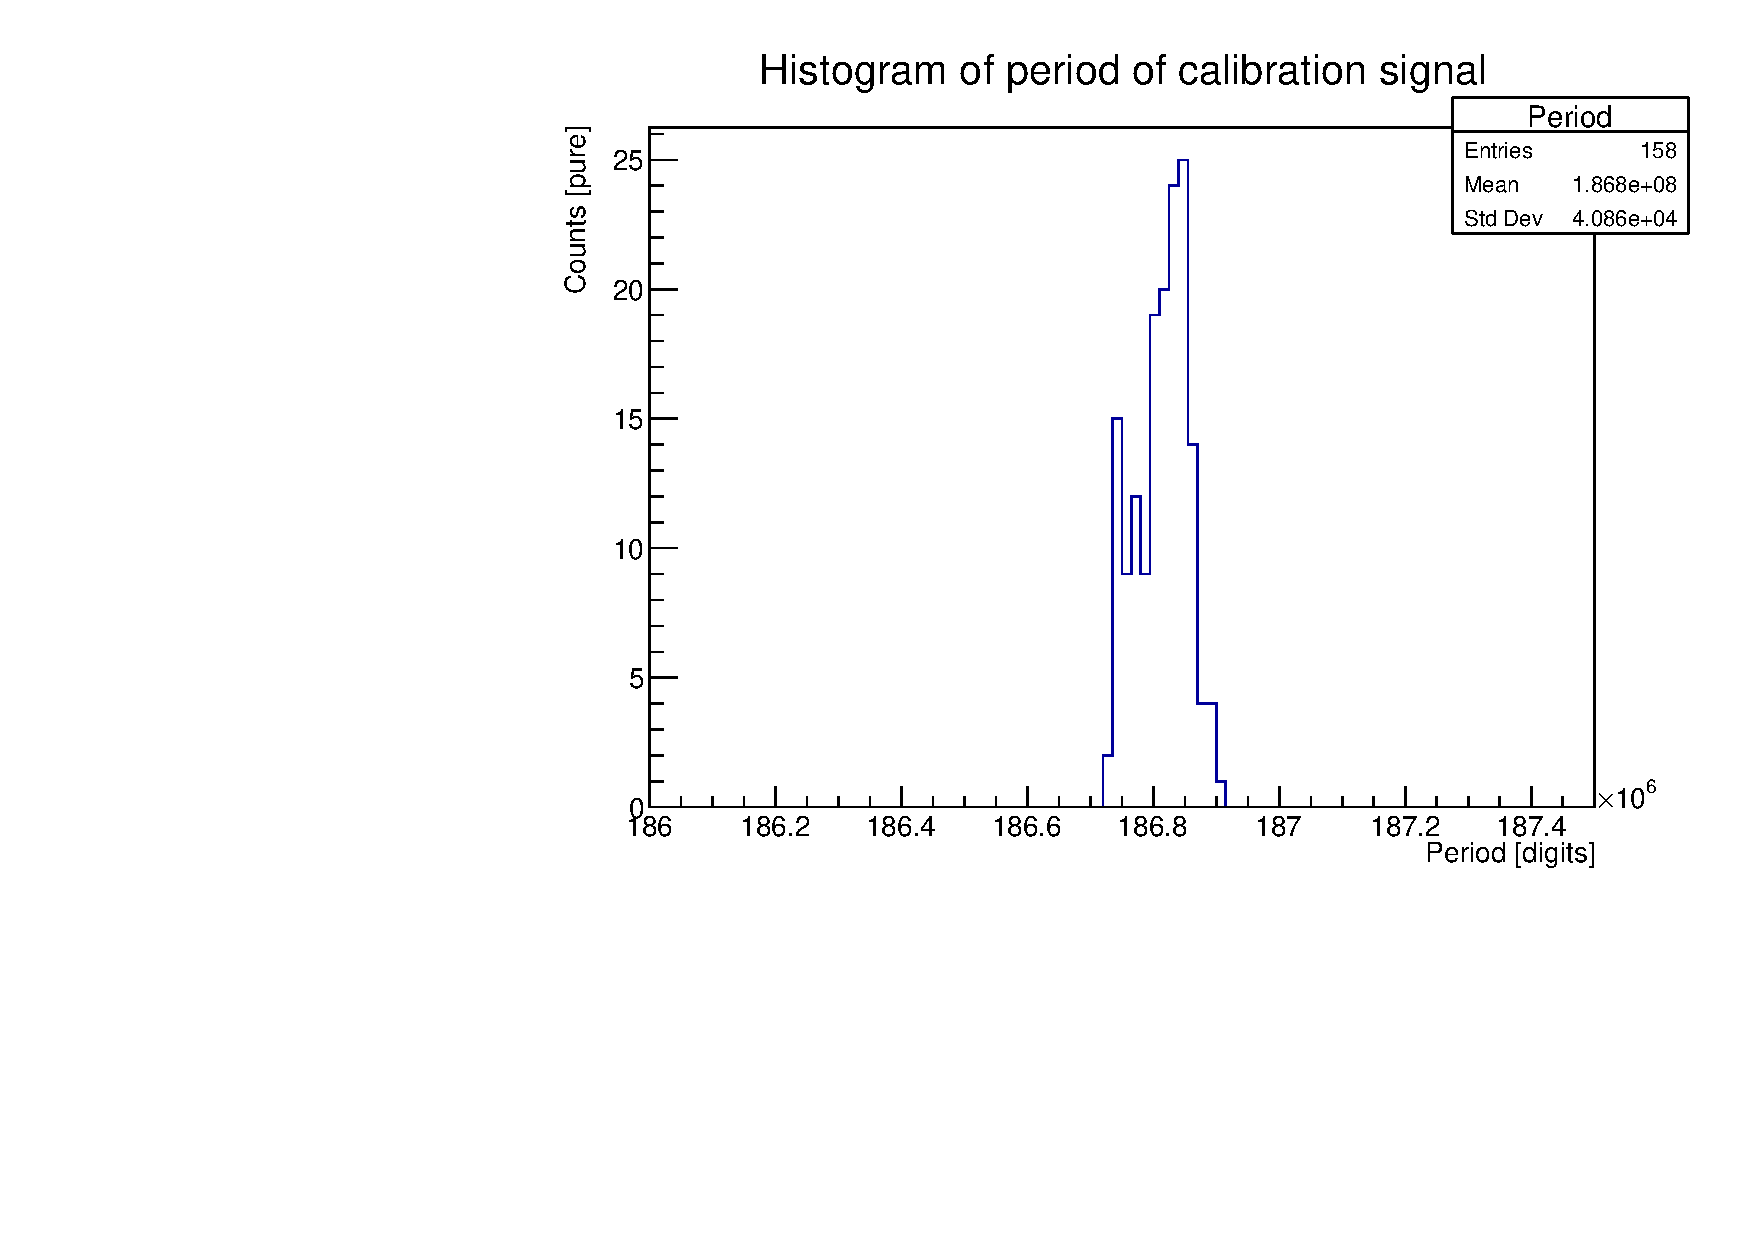
\includegraphics[width=0.7\linewidth]{Grafici/Periodo.pdf}
    \caption{Istogramma periodo del segnale di calibrazione}
    \label{fig:placeholder}
\end{figure}

Quindi, chiamata $\alpha = T[s]/T[dgt]$ la costante di calibrazione, essa vale $\alpha = 4.98892 \pm 0.00002 $ ns/dgt. 

Per completezza abbiamo misurato anche il ritardo fra due canali (lo 0 e l'1), mandando due onde quadre in fase fra loro per vedere se vi era un ritardo dovuto all'acquisizione.

\begin{figure}[H]
    \centering
    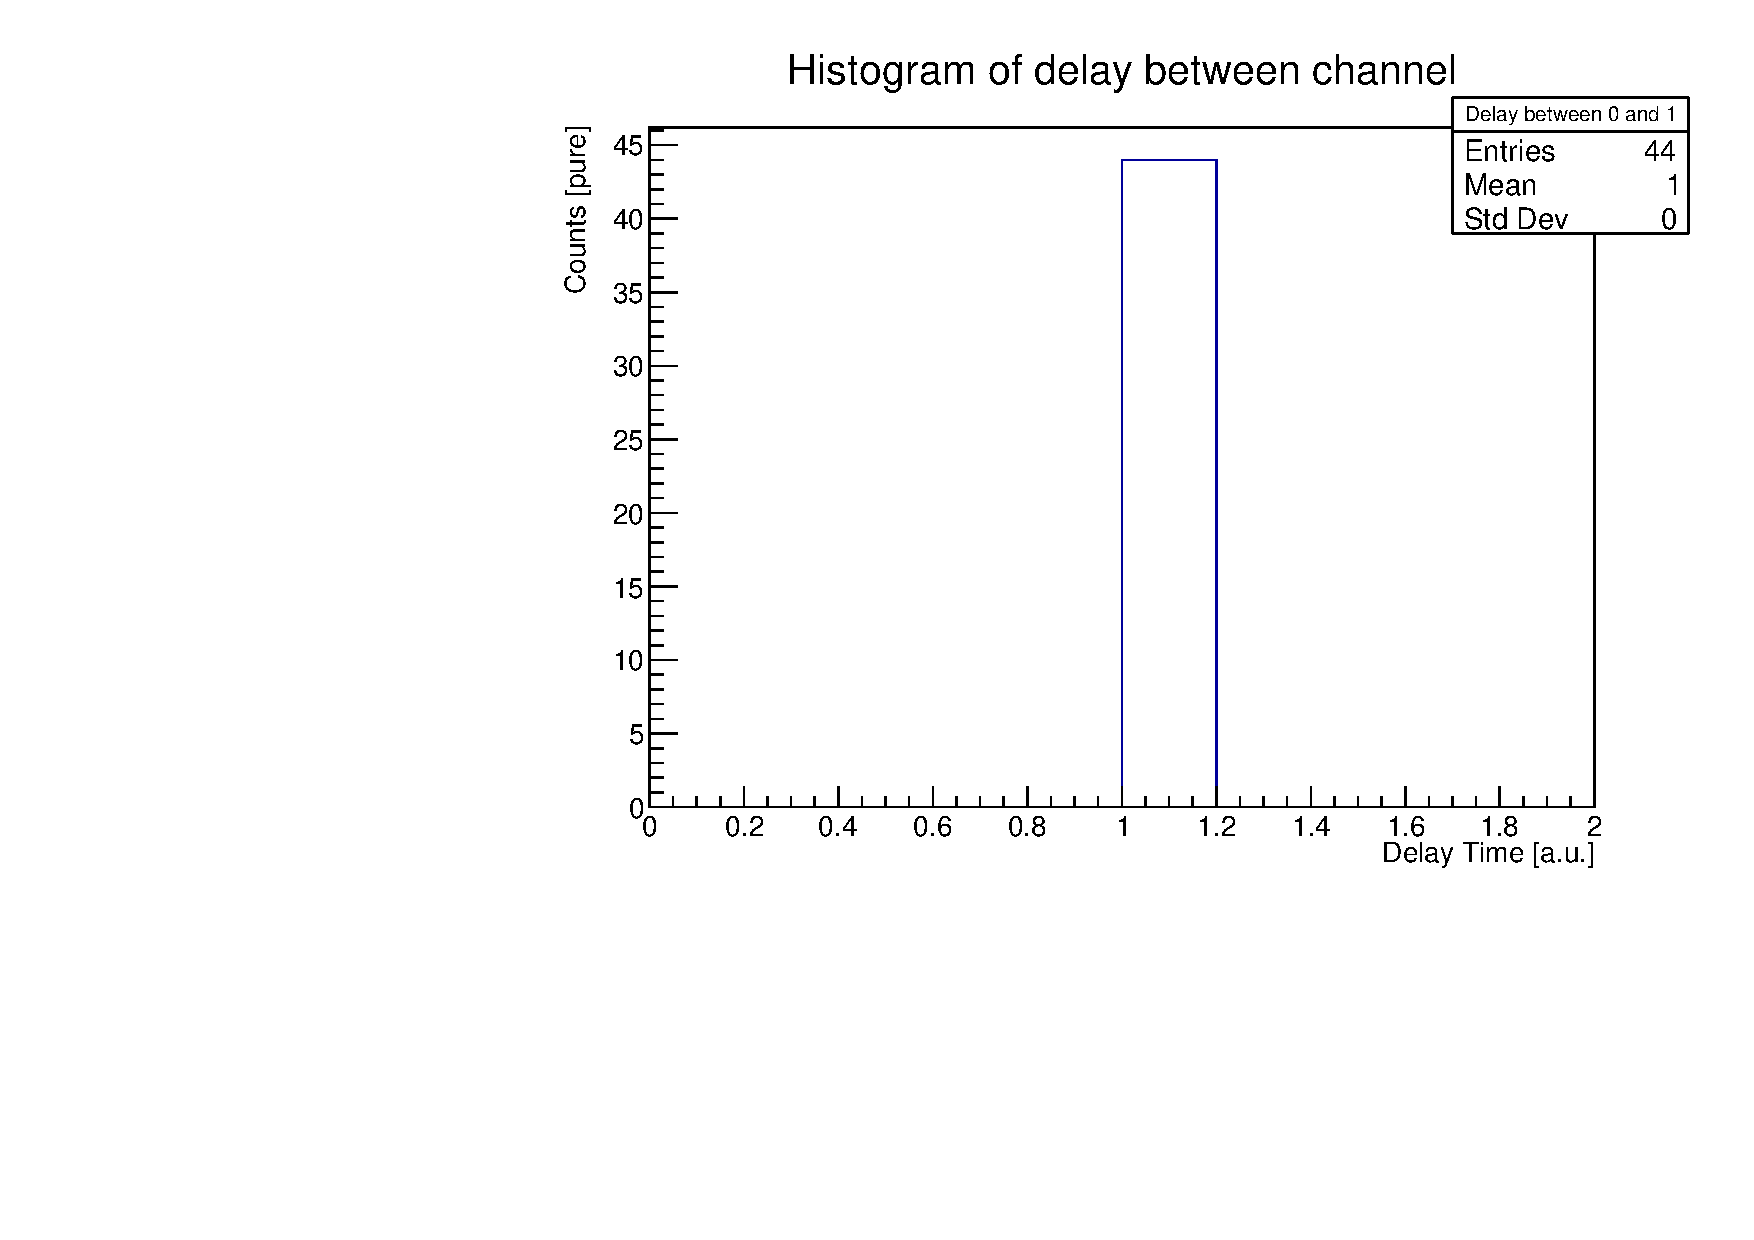
\includegraphics[width=0.7\linewidth]{Grafici/Ritardo.pdf}
    \caption{Istogramma ritardo fra i segnali}
    \label{fig:placeholder}
\end{figure}

Il grafico mostra un digit di differenza fra i due canali, corrispondente al valore di $\alpha$ in nanosecondi.

\section{Misura della vita media}

\subsection{Analisi dati}

Alla scheda abbiamo collegato il segnale di START, il segnale di STOP, e 4 segnali aggiuntivi ottenuti dalla coincidenza del GATE con ciascuno dei PMT08,09,10,11 in OR con il negato del VETO.
Usiamo tali informazioni aggiuntive in sede di analisi dati, al fine di migliorare il riconoscimento dell'evento e rimuovere più eventi di fondo. 

Il nostro algoritmo di analisi dati, funziona nel seguente modo :

\begin{itemize}
\item Individua uno START;
\item Controlla ci sia uno STOP, oppure uno STOP con segnale in uno dei PMT, oppure STOP con segnale in due PMT sovrapposti contemporaneamente;
\item Ripete il controllo cercando i casi precedenti o alternativamente segnale in uno dei PMT;
\item Fa la differenza fra lo START trovato all'inizio e il primo 2.
\end{itemize}

\end{document}